\documentclass{article}

\usepackage {amsmath}
\usepackage[latin1]{inputenc}
\usepackage{tikz}
\usepackage{pgfplots}
\usepackage{color}

\begin{document}
	\title{Matematica Discreta }
	\author{Daniel de la Cruz Prieto}
	\date{\today} 
	
	\maketitle
	
	\paragraph{Definicion}
		Sea $G$ un grafo y A un subconjunto de los vertices de G .El subgrafo de G inducido por A es el subgrafo G(A) , V (G(A))= A 
	
	\begin{equation*}
		\displaystyle E\left(G\left[ A\right]\right)= \left\{e\|e \in E(G), e = <x,y> , x,y \in A\right\}
	\end{equation*}
	
	
	\paragraph{}
	Un subgrafo en expanci\'on $H$ V(H) 
	
	\paragraph{Grafo c\'iclico }
	$C_n$ con $n\geq3$ , $\{V_1,V_2\dots V_n\}$ son los vertices  y $<V_1,V_2>  , <V_2,V_3> \dots <V_n,V_1>$ son las aristas . \\
	Es un grafo regular de grado 2 
	
	\paragraph{} $P_n$ es el grafo de n vertices 
	
	\paragraph{} $K_n$ es el grafo completo (tiene ${n \choose 2 }$ aristas)  
	

	\paragraph{} Grafo de Peterson (Grafo regular de grado 3)
	\begin{center}
		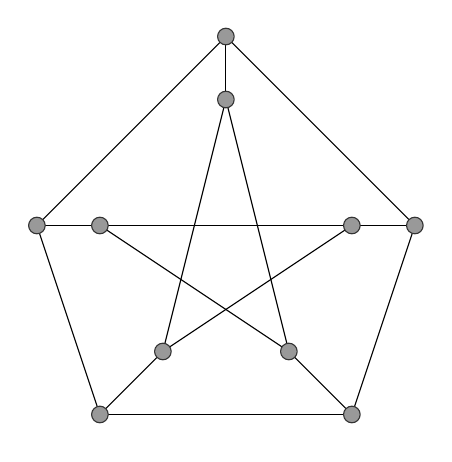
\begin{tikzpicture}[y=.8cm ,x=.80cm]
			\draw (1,0) -- (0,3);
			\draw (1,0) -- (5,0); 
			\draw (5,0) -- (6,3);
			\draw (1,0) -- (2,1);
			\draw (5,0) -- (4,1);
			\draw (0,3) -- (3,6);
			\draw (6,3) -- (3,6);
			\draw (2,1) -- (3,5); 
			\draw (4,1) -- (3,5); 
			\draw (3,5) -- (3,6);
			\draw (4,1) -- (1,3); 
			\draw (2,1) -- (5,3); 
			\draw (1,3) -- (5,3);
			\draw (0,3) -- (1,3);
			\draw (5,3) -- (6,3);
			
			\filldraw[fill=black!40,draw=black!80] (1,0) circle (3pt)    node[anchor=north] {};
			\filldraw[fill=black!40,draw=black!80] (5,0) circle (3pt)    node[anchor=north] {};
			\filldraw[fill=black!40,draw=black!80] (2,1) circle (3pt)    node[anchor=north] {};
			\filldraw[fill=black!40,draw=black!80] (4,1) circle (3pt)    node[anchor=north] {};
			\filldraw[fill=black!40,draw=black!80] (1,3) circle (3pt)    node[anchor=north] {};
			\filldraw[fill=black!40,draw=black!80] (5,3) circle (3pt)    node[anchor=north] {};
			\filldraw[fill=black!40,draw=black!80] (0,3) circle (3pt)    node[anchor=north] {};
			\filldraw[fill=black!40,draw=black!80] (6,3) circle (3pt)    node[anchor=north] {};
			\filldraw[fill=black!40,draw=black!80] (3,6) circle (3pt)    node[anchor=north] {};
			\filldraw[fill=black!40,draw=black!80] (3,5) circle (3pt)    node[anchor=north] {};
			
		\end{tikzpicture}
	\end{center}

	\paragraph{Conjunto independiente } Un connjunto independiente en un grafo $G$ es un conjunto de vertices mutuamente no adyacentes . 
	
	\paragraph{Clique} Un clique en un grafo $G$ es un conjunto de vertices mutuamente adyacentes 
	
	\paragraph{} $\alpha(G)$ es el n\'umero de independencia de $G$
	
	\paragraph{} $ w(G) $ es el n\'umero de clique de $G$
	
	\paragraph{Grafo Bipartito } Un grafo $G$ es bipartito si V(G) es la union de dos conjuntos independientes 
	
	\vspace*{0.5cm}
	\paragraph{Teorema 1}	
	   $G$ es bipartito si no tiene ciclos de longitud impar 
	    
	\subsection*{Demostracion} 
	 
	\hspace*{0.5cm} 
	$\Rightarrow$ Si el grafo es bipartito entonces se puede biparticionar en los conjuntos $A$ y $B$ tal que todas las aristas van del conjunto $A$ al $B$  y/o  viceversa . Luego no pueden existir ciclos de longitud impar. Pues supongamos que el ciclo $C$ que tomando uno de los v\'ertices que lo compone ,llamemoslo $v$ , todo recorrido es posible hacerlo partiendo de $v$ y sin perdida de generalidad vamos a asumir que el vertice $v$ esta en el conjunto $A$ , luego cualquier recorrido que se haga tiene que comenzar en $A$ y terminar en $A$ , luego como las aristas de $G$ van solo de un conjunto a otro y no hay aristas que vayan de un conjunto hacia el mismo . Por lo que todo recorrido que empice en $A$ y termine en $A$ tiene longitud  par , luego $C$ no puede ser de longitud impar 
	
	\vspace*{0.3cm}
	$\Leftarrow$ Ahora vamos a demostrar que si el grafo no tiene ciclos de longitud impar entonces se puede biparticionar .
	Vamos a hacerlo por induccion fuerte en la cantidad de v\'ertices del grafo . Vamos a asumir que el grafo es conexo para apoyarnos en la hipotesis de induccion , seria de la siguiente manera , dado un grafo conexo que no tiene ciclos de longitud impar entonces se puede biparticionar , si el grafo no fuera conexo no importaria porque ahora dadas todas sus componentes conexas , si estas se pueden biparticionar entonces se pueden repartir las biparticiones de forma tal que el grafo se puede biparticionar de forma tal que no haya incongruencia en su biparticion .
	
	Dado un grafo $G$ de $n+1$ v\'ertices conexo y que no tiene ciclos de longitud impar entonces el grafo es bipartito . 
	
	Vamos a quitarle un v\'ertice $v$ al grafo $G$, ahora se nos formo el grafo $G'$ de n vertices , pero por hipotesis de induccion el grafo $G'$ es bipartito , pero el grafo $G'$ se pudo haber desconectado al haberle quitado el v\'ertice $v$ al grafo $G$ (a la hora de construirlo) . Sean ahora $C_1',C_2'\dots C_k'$ las componentes conexas de $G'$ . Estas componentes conexas cada una se puede biparticionar en los conjuntos $c_{i_a}'$ y $c_{i_b}' $ cada una .Ahora poniendo a $v$ de vuelta en el grafo tenemos de que $v$ tiene adyacentes en cada una de las componenetes conexas porque $G$ es conexo  , tambien se cumple que $v$ solo pude tener edyacentes en uno y solo una de las particiones de las componentes conexas de $G'$ porque si tuviera en ambos lados de la biparticion de cada una de la componentes conexas existirian ciclos de longitud impar , lo que no pude pasar porque yo habia asumido que en $G$ no habian ciclos de longitud impar , luego puedo encontrar una biparticion de $G$ , luego queda demostrado el teorema 
	
	 
	
	
	

\end{document}